\par As described above, diKTat is configurable and user-friendly. But these are not all of it's advantages and features. Below we will present and describe unusual and important killer-features of diKTat.

\subsection{Configuration file}
\par
It's worth starting with the configuration file. This is a file in which the user can manually turn rules on and off or configure the rules settings. Below is one of the rules in the configuration file.
\\
\begin{lstlisting}[ caption={Part of configuration file.},
label={lst:example1}, language=yaml]
- name: DIKTAT_COMMON
  configuration:
    # put your package name here - it will be autofixed and checked
    domainName: your.name.here
- name: COMMENTED_OUT_CODE
  enabled: true
- name: HEADER_MISSING_OR_WRONG_COPYRIGHT
  enabled: true
  configuration:
    isCopyrightMandatory: true
    copyrightText: 'Copyright (c) Your Company Name Here. 2010-2020'
    testDirs: test
- name: FILE_IS_TOO_LONG
  enabled: true
  configuration:
    maxSize: '2000'
    ignoreFolders: ' '
\end{lstlisting}
Each Inspection in this file has 3 fields: \texttt{name} - the name of the Inspection, \texttt{enabled} - whether the rule is enabled or disabled (all rules are enabled by default), \texttt{configuration} - parameters for the Inspection. With the first two, everything is obvious. The third parameter is less obvious. The configuration is a set of "properties" to configure this rule. For example, for an Inspection \texttt{FILE\underline{ }IS\underline{ }TOO\underline{ }LONG}, that checks the number of lines in a Kotlin file, the user can configure the maximum number of lines allowed in the file - by changing the "maxSize" in the configuration, or the user can specify paths to folders that do not need to be checked - by writing the path in "ignoreFolders". \\

\subsection{Create ASTNode}
Another feature is a special mechanism that allows you to construct an abstract syntax tree node from the text. It is extremely useful for creating automatic fixers, because you do not need to think about the AST implementation and you simply need to provide a text block with a code. Everything will be done under the hood by the framework. This algorithm can parse the code even partially, when you do not need to save the hierarchy of the file (with imports/packages/classes).
For example it can parse and provide you a sub-tree for these lines of code:

\begin{lstlisting}[caption={Example of creating an AST from text of code.}, label={lst:example1}, language=Kotlin]
	val nodeFromText: ASTNode = KotlinParser().createNode("val age: Int = 21")
\end{lstlisting}

\tikzstyle{every node}=[draw=black,thick,anchor=west, scale = 0.5]
  
\begin{tikzpicture}[%
  grow via three points={one child at (0.3,-0.8) and
  two children at (0.3,-0.8) and (0.3,-1.5)},
  scale=0.5,
  edge from parent path={(\tikzparentnode.south) |- (\tikzchildnode.west)}]
    
  \node {PROPERTY}
    child { node {val}}
    child {node {WHITE\underline{ }SPACE}}
    child {node {IDENTIFIER}}
    child {node {COLON}}
    child {node {WHITE\underline{ }SPACE}}
    child {node {TYPE\underline{ }REFERENCE}
    	child {node {USER\underline{ }TYPE}
		child {node {REFERENCE\underline{ }EXPRESSION}
			child {node {IDENTIFIER}}
		}
	}
    }
    child [missing] {}
    child [missing] {}
    child [missing] {}  
    child {node {WHITE\underline{ }SPACE}}
    child {node {EQ}}
    child {node {WHITE\underline{ }SPACE}}
    child {node {INTEGER\underline{ }CONSTANT}
    	child {node {INTEGER\underline{ }LIRETAL}}
    };
\end{tikzpicture}
\\

As you can see in the example, we pass the text of the source code, that we want to transform, to the method.  What's going on inside this method? First of all, special system properties (used by Kotlin parser) are set (for example: set "idea.io.use.nio2" to true). If the text of the code contains high-level keywords like \texttt{import} or \texttt{package}, then the method builds a tree with a root node of the FILE type, otherwise it tries with a different root type. In both cases, at the end, if the tree contains a node with type \texttt{ERROR\underline{ }ELEMENT}, it means that some of the code and the method was unable to build the tree and, therefore, throws an exception.\\
This helps us to implement such complex inspections like the detection of commented code (and distinguish real comments from commented code blocks), helps easily fix the code without manually building sub-trees in visitors.\\

\subsection{Suppress annotation}
\par
What if the user wants one of the diKTat Inspections not to check a particular piece of code? The \textsl{SUPPRESS} annotation will help us with it. This annotation can be used to ignore a certain Inspection in a certain code block. For instance, if we run this code:

\begin{lstlisting}[caption={Function with incorrect name.}, label={lst:example1}, language=Kotlin]
/**
 * This is example
 */

package org.cqfn.diktat

/**
 * Simple class
 */
class User(private val name: String, private val age: Int) {
	/**
	 * Function with incorrect name
	 *
	 * @return is username longer than age
	 */
	fun IsInCoRrEcTnAMe() = name.length > age
}

\end{lstlisting}

Diktat will raise the warning: 
$$
\texttt{ \small{ $\big[$FUNCTION\underline{ }NAME\underline{ }INCORRECT\underline{ }CASE$\big]$  function/method name should be in lowerCamelCase}}
$$

But if there is a \texttt{@Suppress} before this method, then there will be no warnings during the run:
\begin{lstlisting}[caption={Function with incorrect name, but with suppressed Inspection.}, label={lst:example1}, language=Kotlin]
/**
 * This is example
 */

package org.cqfn.diktat

/**
 * Simple class
 */
@Suppress("FUNCTION_NAME_INCORRECT_CASE")
class User(private val name: String, private val age: Int) {
	/**
	 * Function with incorrect name
	 *
	 * @return is username longer than age
	 */
	fun IsInCoRrEcTnAMe() = name.length > age
}

\end{lstlisting}

The example shows that the method has a suppress annotation. Therefore, the \texttt{FUNCTION\underline{ }NAME\underline{ }INCORRECT\underline{ }CASE} rule will be ignored on this method and there will be no error. The search method for a given annotation goes up recursively to the root element of type \texttt{FILE}, looking for the annotation. This means that \texttt{@Suppress} can be placed not only in front of knowingly incorrect code, but also at the upper levels of the abstract syntax tree. In our example, the annotation is not in front of the method, but in front of the class and it still works. Also, you can put several annotations:
\begin{lstlisting}[caption={Several suppression annotations}, label={lst:example1}, language=Kotlin]
@set:[Suppress("WRONG_DECLARATION_ORDER") Suppress("IDENTIFIER_LENGTH")]
\end{lstlisting}

\subsection{WEB}
It worth mentioning that there is a web version of diKTat. This is a handy tool that can be used quickly without any installations, and it is very simple. The link can be found in or you can find it in "\nameref{sec:download}" chapter or in ktlint project as reference.\footnote{\url{https://github.com/pinterest/ktlint\#online-demo}}
\begin{figure}[H]
  \centering
  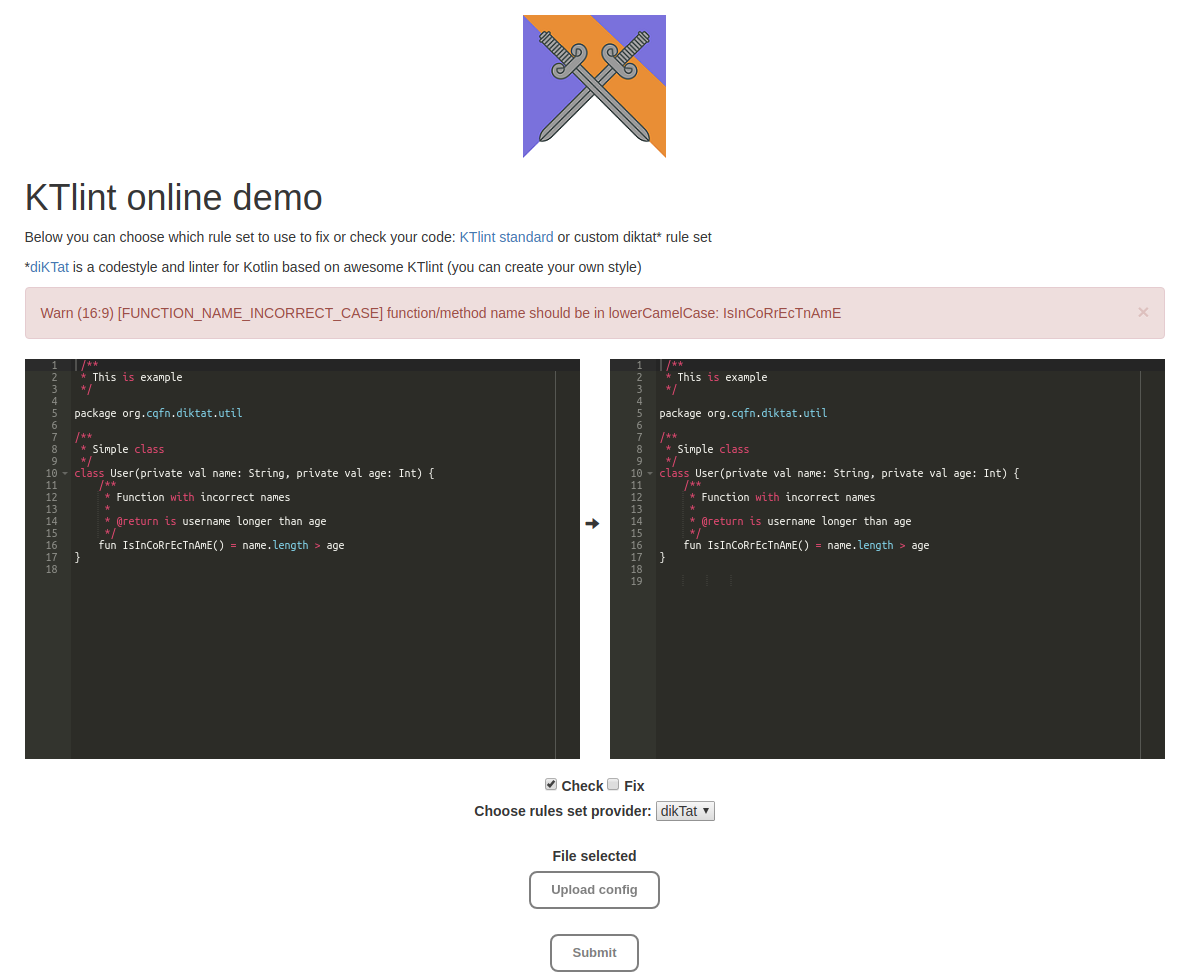
\includegraphics[scale=0.3]{pictures/web-example.png}
  \caption{Diktat-web online demo} 
\end{figure} 

\subsection{Options validation}
As it has been mention earlier, diktat has a highly customizable configuration file, but manually editing it is error-prone, for example, name of the rule can be incorrect due to a typo. Diktat will validate configuration file on startup and suggest the closest name based on \textsl{Levenshtein} method.

\subsection{Self checks}
Diktat fully supports self checking of it's own code using both release and snapshot (master) versions. Diktat uses it's self to validate the code inside during it's CI/CD process. 
